\chapter{Planos de Distribución Física y Cuadro Consolidado de Materiales}

\section{Introducción al Diseño Físico}

La presente etapa consolida la representación gráfica de ingeniería y la valoración económica de la infraestructura física del Policlínico ``Salud \& Vida''. El diseño físico está modelado a escala exacta \textbf{1:100} en el sistema interactivo SVG (\texttt{plano/index.html}), descompuesto en cuatro capas vectoriales independientes:

\begin{enumerate}[leftmargin=*, label=\arabic*.]
    \item \textbf{Capa 1:} Arquitectura y tabiquería (muros de 15~cm, puertas y losa).
    \item \textbf{Capa 2:} Tomas de usuario y puntos de conexión (56 jacks RJ-45).
    \item \textbf{Capa 3:} Canalizaciones físicas (bandeja tipo malla + canaleta PVC de dos vías).
    \item \textbf{Capa 4:} Células de cobertura WLAN Wi-Fi~6 (radios de 8.0~m a 5~GHz).
\end{enumerate}

\begin{figure}[H]
\centering
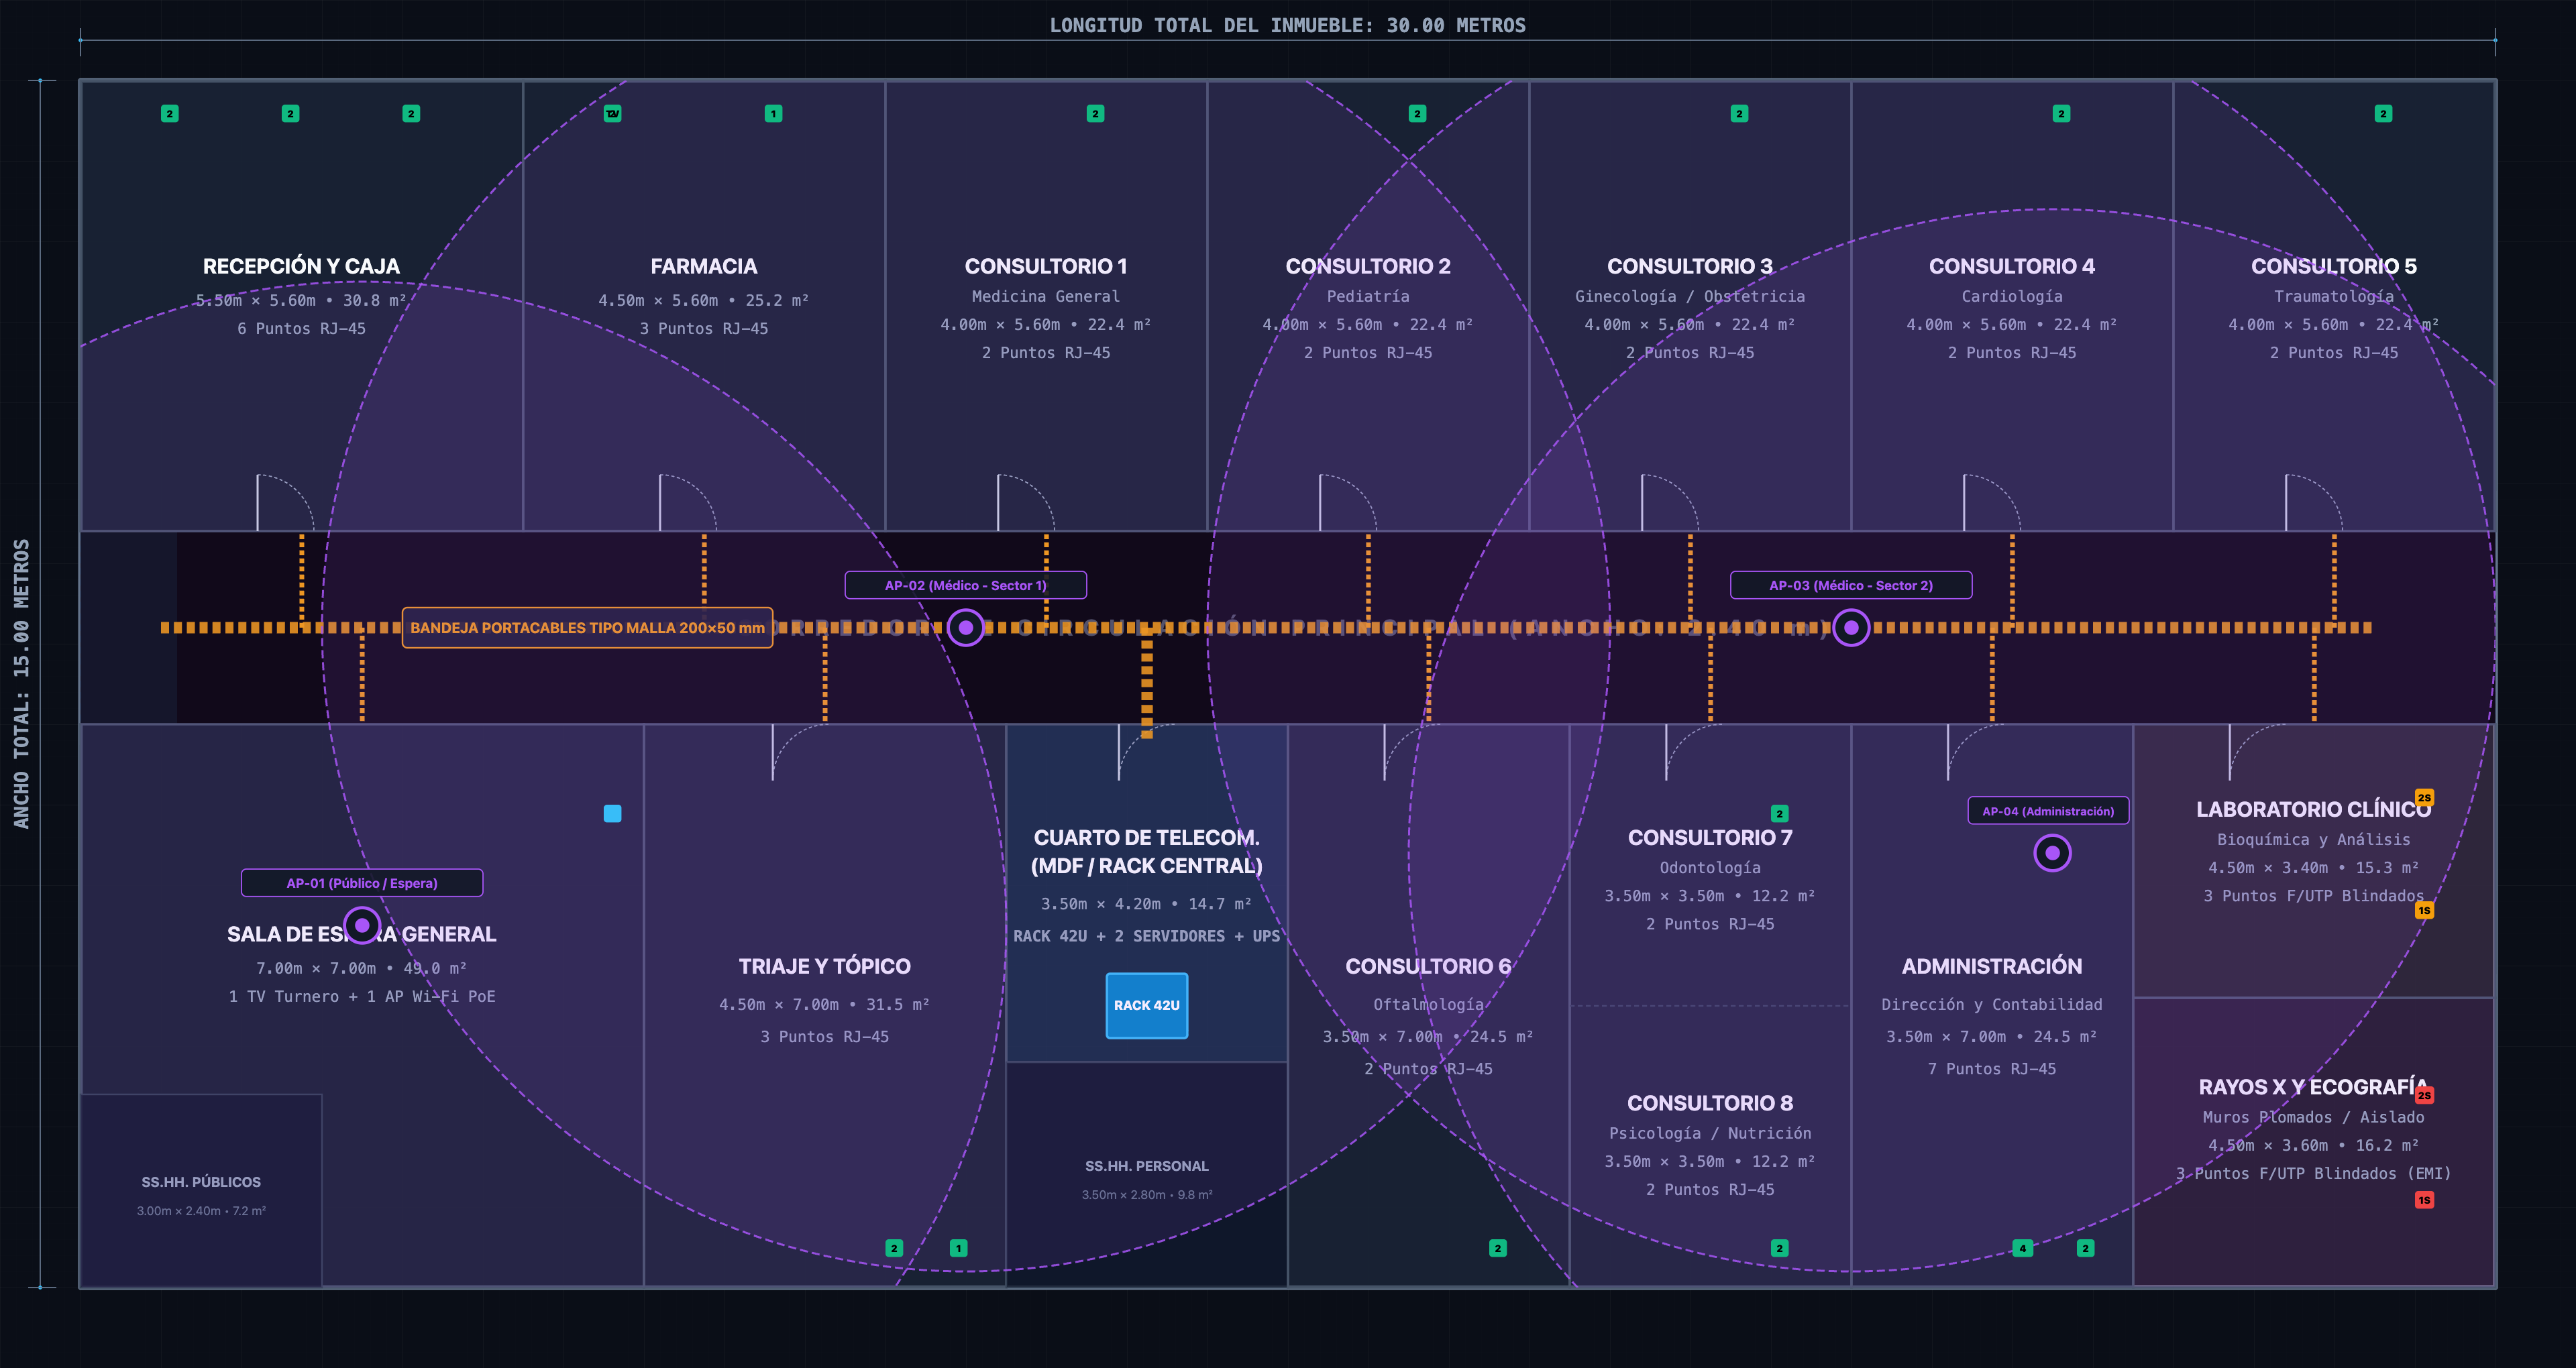
\includegraphics[width=\textwidth]{plano.png}
\caption{Plano arquitectónico civil y distribución espacial de ambientes del Policlínico (Escala 1:100)}
\label{fig:plano-civil}
\end{figure}

\begin{figure}[H]
\centering
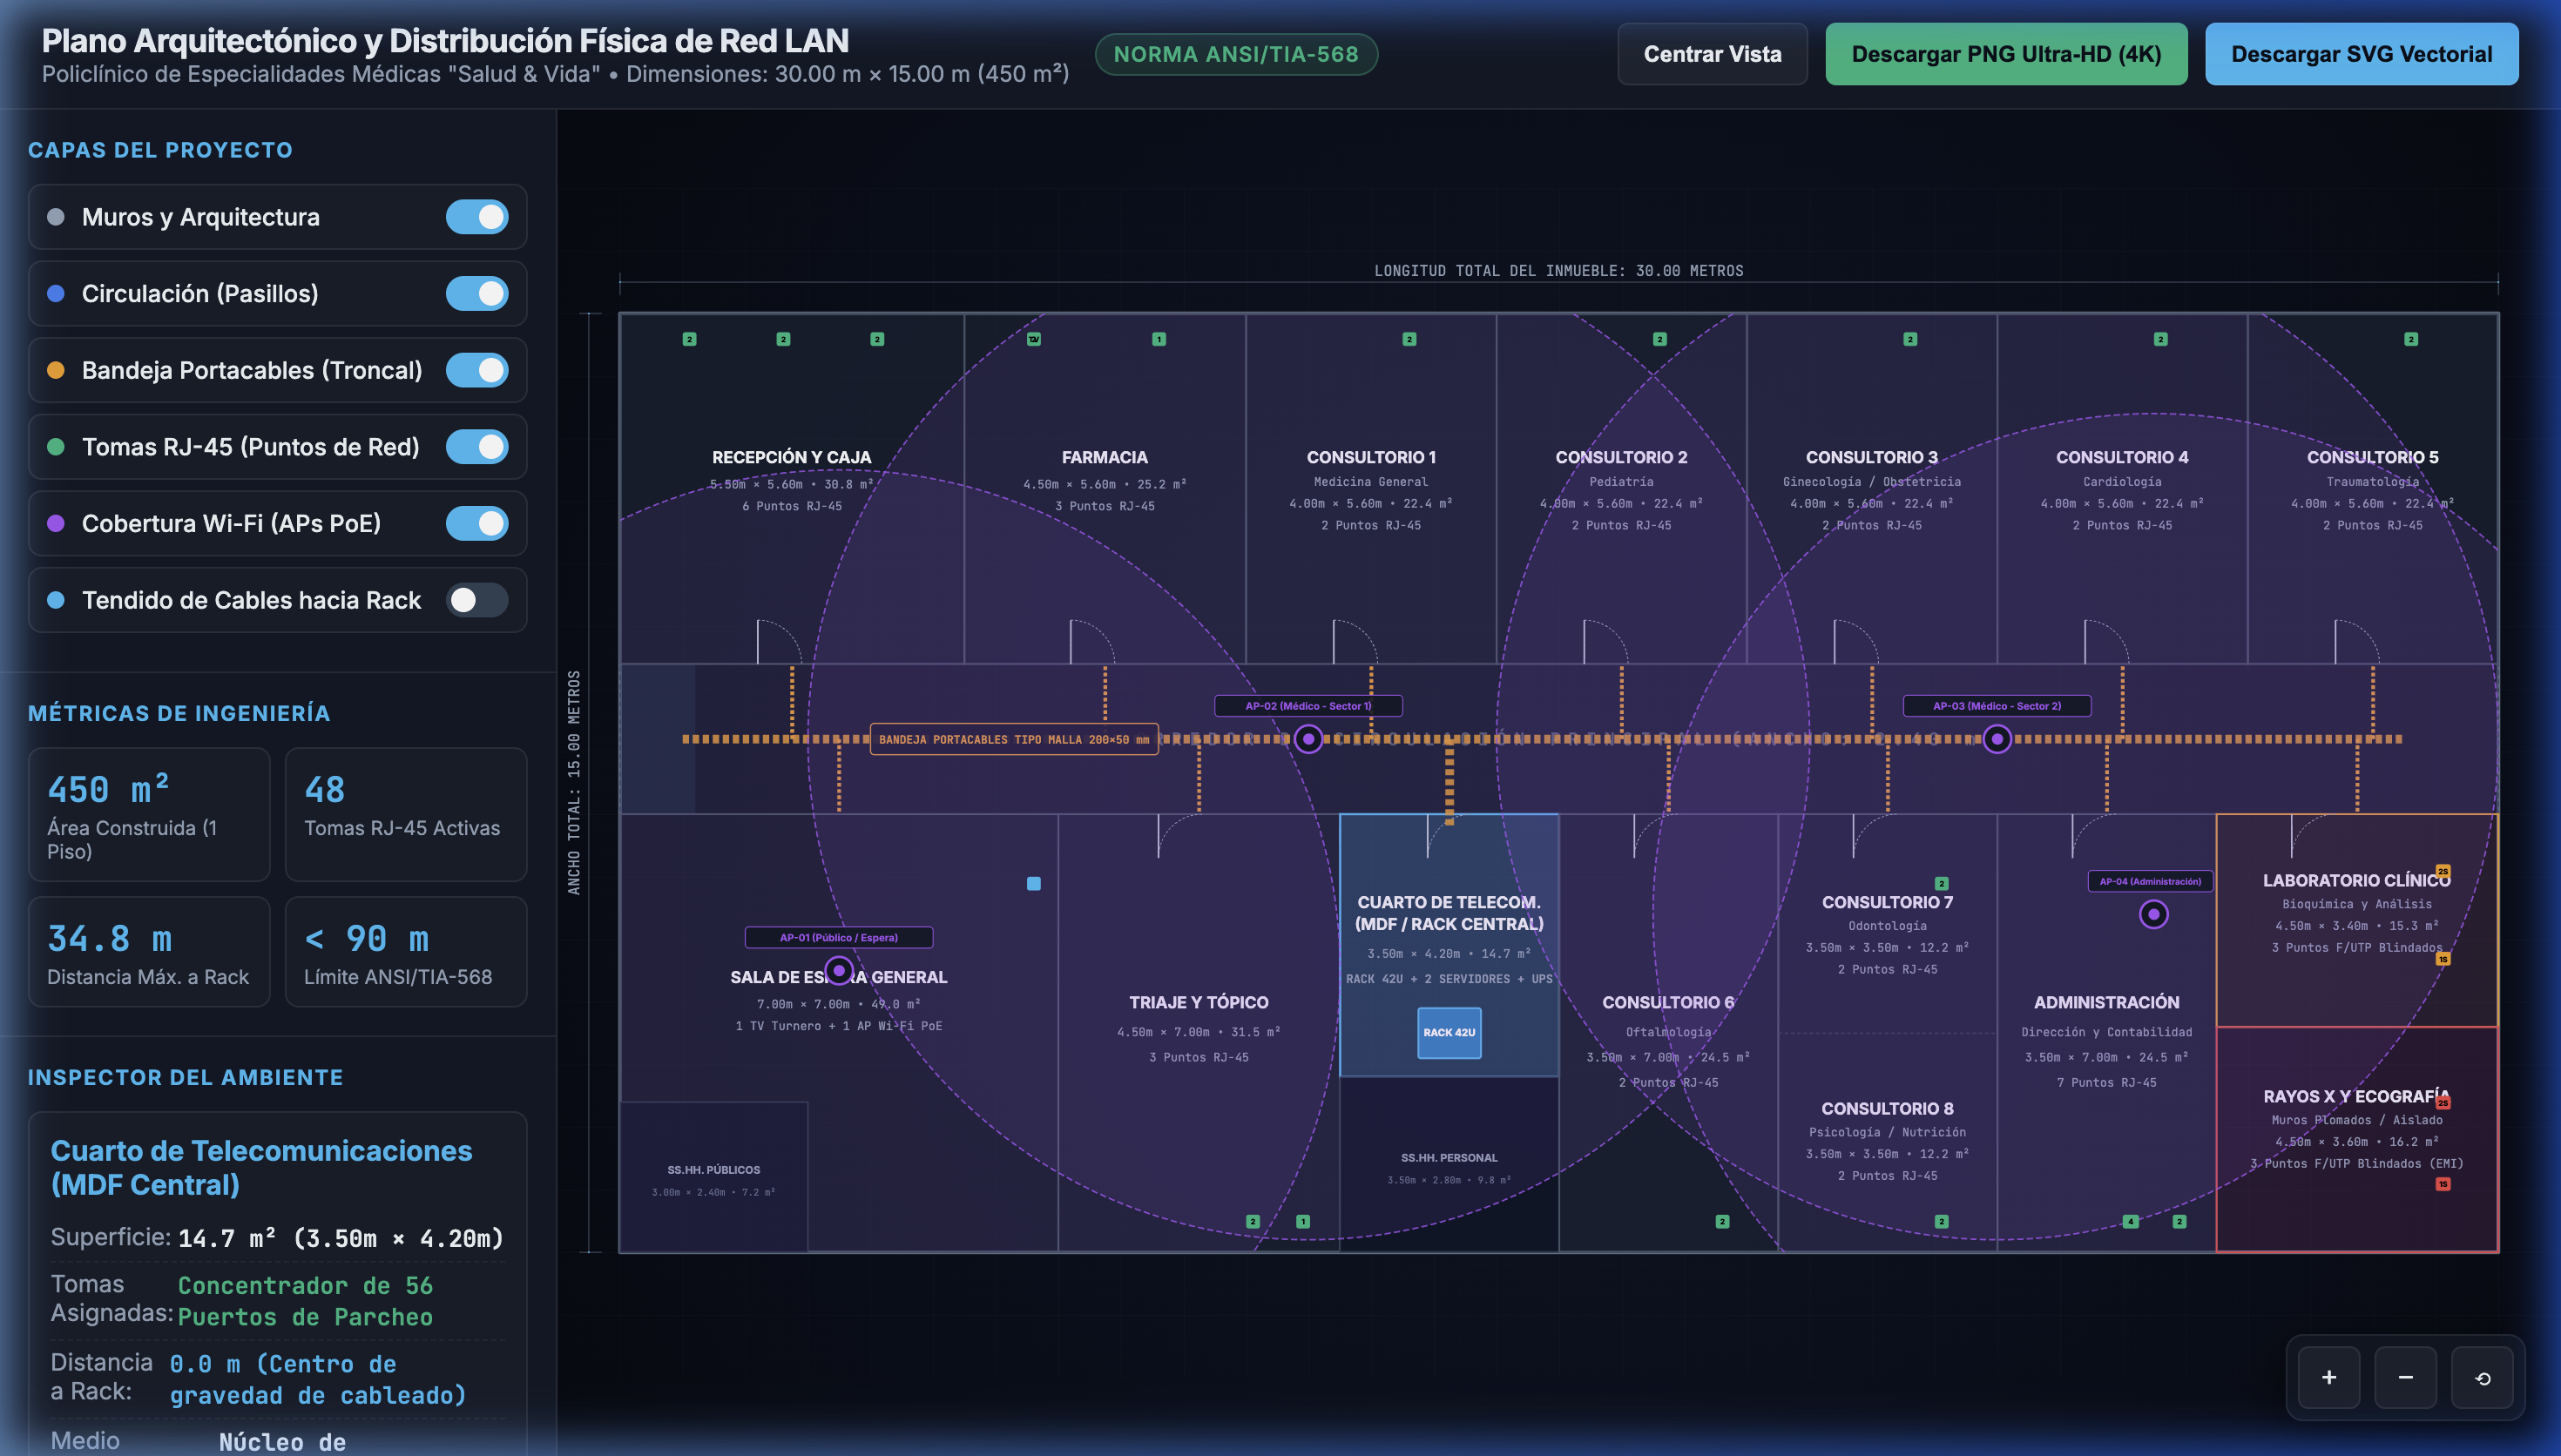
\includegraphics[width=\textwidth]{plano_red_preview.png}
\caption{Plano integral de ingeniería de red LAN: cableado estructurado, canalizaciones y celdas Wi-Fi~6}
\label{fig:plano-red-completo}
\end{figure}

\section{Simbología Normalizada ANSI/TIA-606-B}

\begin{table}[H]
\centering
\caption{Simbología técnica normalizada para planos de red}
\begin{tabularx}{\textwidth}{@{}cclX@{}}
\toprule
\textbf{Símbolo} & \textbf{Código TIA} & \textbf{Componente} & \textbf{Ubicación y Altura} \\
\midrule
$[\bullet\ \bullet]$ & TO-UTP-2  & Toma doble RJ-45 Cat~6 UTP      & Pared a +0.40~m s.n.p.t. / +1.10~m en mesadas \\
$[\blacksquare\ \blacksquare]$  & TO-FTP-2  & Toma doble RJ-45 Cat~6A F/UTP   & Pared a +1.10~m en Lab. y Rayos~X, con tierra \\
$((\text{AP}))$      & WLAN-AP   & Access Point Wi-Fi~6 PoE+       & Anclado en cielo raso a +2.60~m \\
$[\text{TV}]$        & TO-IPTV   & Toma RJ-45 para Smart TV Turnos & Mural a +1.80~m en Sala de Espera \\
$[\text{Rack 42U}]$  & MDF-R1    & Gabinete Rack 42U principal     & Centro geográfico, fijado en losa de concreto \\
$\equiv$             & PATH-BM   & Bandeja malla 200$\times$50~mm  & Suspendida en falso techo a +2.75~m (pasillo) \\
$-\,-\,-$            & PATH-CP   & Canaleta PVC 2 vías 40$\times$25~mm & Adosada a muros a +0.40~m s.n.p.t. \\
\bottomrule
\end{tabularx}
\label{tab:simbologia}
\end{table}

\section{Matriz de Coordenadas y Distancias por Ambiente}

\begin{table}[H]
\centering
\caption{Distancias de enlace permanente por ambiente respecto al MDF}
\small
\begin{tabularx}{\textwidth}{@{} c X c c c c @{}}
\toprule
\textbf{N°} & \textbf{Ambiente} & \textbf{Dim. (m)} & \textbf{Tomas} & \textbf{Dist. Horiz.} & \textbf{Enl. Perm.} \\
\midrule
01 & Recepción / Admisión / Caja        & 5.5$\times$5.6 & 6 UTP   & 13.50~m & 17.70~m \\
02 & Sala de Espera General             & 7.0$\times$7.0 & 2 UTP   & 10.00~m & 14.20~m \\
03 & Triaje y Tópico                    & 4.5$\times$7.0 & 3 UTP   &  6.50~m & 10.70~m \\
04 & Consultorio 01 (Medicina General)  & 4.0$\times$5.6 & 2 UTP   &  4.80~m &  9.00~m \\
05 & Consultorio 02 (Pediatría)         & 4.0$\times$5.6 & 2 UTP   &  6.30~m & 10.50~m \\
06 & Consultorio 03 (Ginecología)       & 4.0$\times$5.6 & 2 UTP   & 10.30~m & 14.50~m \\
07 & Consultorio 04 (Cardiología)       & 4.0$\times$5.6 & 2 UTP   & 14.30~m & 18.50~m \\
08 & Consultorio 05 (Traumatología - Extremo Este) & 4.0$\times$5.6 & 2 UTP & 18.30~m & 22.50~m \\
09 & Consultorio 06 (Oftalmología)      & 3.5$\times$7.0 & 2 UTP   &  6.50~m & 10.70~m \\
10 & Consultorio 07 (Odontología)       & 3.5$\times$3.5 & 2 UTP   &  9.00~m & 13.20~m \\
11 & Consultorio 08 (Psicología)        & 3.5$\times$3.5 & 2 UTP   & 12.00~m & 16.20~m \\
12 & Rayos~X y Ecografía (Zona Crítica) & 4.5$\times$3.6 & 3 F/UTP & 21.00~m & 25.20~m \\
13 & Lab. Clínico (Zona Crítica)        & 4.5$\times$3.4 & 3 F/UTP & 22.00~m & \textbf{34.80~m}$^*$ \\
14 & Farmacia Asistencial               & 4.5$\times$5.6 & 3 UTP   &  9.00~m & 13.20~m \\
15 & Administración / Jefatura          & 3.5$\times$7.0 & 7 UTP   & 15.00~m & 19.20~m \\
16 & Pasillo Central (AP-02 y AP-03)    & 30.0$\times$2.4& 2 PoE   &  7.00~m &  8.50~m \\
17 & Rack MDF (Servidores directos)     & 3.5$\times$4.2 & 3 F/UTP &  1.50~m &  2.50~m \\
18 & Reservas técnicas (distribuidas)   & ---            & 8 UTP   & 18.00~m & 22.20~m \\
\midrule
\multicolumn{3}{l}{\textbf{Total}} & \textbf{56 Tomas} & --- & \textbf{Prom.: 16.5~m} \\
\bottomrule
\multicolumn{6}{@{}p{\textwidth}@{}}{\footnotesize $^*$Toma más lejana (extremo este con retorno ordenado por bandeja). Límite normativo ANSI/TIA-568: $\leq 90.0$~m. Margen de seguridad: +55.2~m (61.3\%).} \\
\end{tabularx}
\label{tab:distancias}
\end{table}

\begin{figure}[H]
\centering
\begin{tikzpicture}[scale=0.45, every node/.style={transform shape}]
    % Perímetro exterior del edificio (30.0m x 15.0m a escala real)
    \draw[line width=1.8pt, fill=gray!3] (0,0) rectangle (30, 15);
    
    % Pasillo central de circulación (X: 0 a 30m, Y: 7.0 a 9.4m -> Ancho 2.4m)
    \draw[fill=yellow!10, draw=gray!40] (0, 7.0) rectangle (30, 9.4);
    \node[font=\bfseries\tiny, text=gray!60] at (15, 8.9) {PASILLO CENTRAL DE CIRCULACIÓN (30.0~m $\times$ 2.4~m)};

    % ========================================================
    % ALA NORTE (Y: 9.4m a 15.0m, Fondo 5.6m) - De Oeste a Este
    % ========================================================
    % 1. Recepción y Caja (0 a 5.5m)
    \draw[line width=1pt, fill=blue!10] (0, 9.4) rectangle (5.5, 15.0);
    \node[align=center, font=\scriptsize\bfseries] at (2.75, 12.2) {RECEPCIÓN\\Y CAJA\\{\tiny 5.5$\times$5.6m}\\{\tiny\color{blue!80!black} 6 Tomas UTP}};

    % 2. Farmacia Asistencial (5.5 a 10.0m)
    \draw[line width=1pt, fill=blue!5] (5.5, 9.4) rectangle (10.0, 15.0);
    \node[align=center, font=\scriptsize] at (7.75, 12.2) {\textbf{FARMACIA}\\{\tiny 4.5$\times$5.6m}\\{\tiny 3 Tomas UTP}};

    % 3. Consultorio 01 - Medicina General (10.0 a 14.0m)
    \draw[line width=1pt] (10.0, 9.4) rectangle (14.0, 15.0);
    \node[align=center, font=\scriptsize] at (12.0, 12.2) {\textbf{C-01}\\{\tiny Med. General}\\{\tiny 4.0$\times$5.6m}\\{\tiny 2 UTP}};

    % 4. Consultorio 02 - Pediatría (14.0 a 18.0m)
    \draw[line width=1pt] (14.0, 9.4) rectangle (18.0, 15.0);
    \node[align=center, font=\scriptsize] at (16.0, 12.2) {\textbf{C-02}\\{\tiny Pediatría}\\{\tiny 4.0$\times$5.6m}\\{\tiny 2 UTP}};

    % 5. Consultorio 03 - Ginecología / Obstetricia (18.0 a 22.0m)
    \draw[line width=1pt] (18.0, 9.4) rectangle (22.0, 15.0);
    \node[align=center, font=\scriptsize] at (20.0, 12.2) {\textbf{C-03}\\{\tiny Ginecología}\\{\tiny 4.0$\times$5.6m}\\{\tiny 2 UTP}};

    % 6. Consultorio 04 - Cardiología (22.0 a 26.0m)
    \draw[line width=1pt] (22.0, 9.4) rectangle (26.0, 15.0);
    \node[align=center, font=\scriptsize] at (24.0, 12.2) {\textbf{C-04}\\{\tiny Cardiología}\\{\tiny 4.0$\times$5.6m}\\{\tiny 2 UTP}};

    % 7. Consultorio 05 - Traumatología (Extremo Este) (26.0 a 30.0m)
    \draw[line width=1pt] (26.0, 9.4) rectangle (30.0, 15.0);
    \node[align=center, font=\scriptsize] at (28.0, 12.2) {\textbf{C-05}\\{\tiny Traumatología}\\{\tiny 4.0$\times$5.6m}\\{\tiny 2 UTP}};

    % ========================================================
    % ALA SUR (Y: 0.0m a 7.0m, Fondo 7.0m) - De Oeste a Este
    % ========================================================
    % 8. Sala de Espera General (0 a 7.0m, Y: 0 a 7.0m)
    \draw[line width=1pt, fill=purple!5] (0, 0) rectangle (7.0, 7.0);
    \draw[fill=gray!25, draw=gray!60] (0, 0) rectangle (3.0, 2.4);
    \node[font=\tiny\bfseries, text=gray!70] at (1.5, 1.2) {SS.HH. PÚBL.};
    \node[align=center, font=\scriptsize\bfseries] at (4.8, 5.5) {SALA DE ESPERA\\GENERAL\\{\tiny 7.0$\times$7.0m (49~m$^2$)}\\{\tiny 2 UTP + Smart TV}};
    % AP-01 UBICADO EXACTAMENTE EN SALA DE ESPERA GENERAL
    \node[circle, fill=purple, text=white, inner sep=2.2pt, font=\bfseries\tiny] (ap1) at (4.0, 3.6) {AP1};
    \draw[purple, dashed, line width=0.9pt] (4.0, 3.6) circle (3.2cm);
    \node[font=\tiny\bfseries, text=purple!90!black, fill=white, inner sep=1pt] at (4.0, 2.9) {AP-01 (Público/Espera)};

    % 9. Triaje y Tópico de Urgencias (7.0 a 11.5m)
    \draw[line width=1pt] (7.0, 0) rectangle (11.5, 7.0);
    \node[align=center, font=\scriptsize] at (9.25, 3.5) {\textbf{TRIAJE Y}\\\textbf{TÓPICO}\\{\tiny 4.5$\times$7.0m}\\{\tiny 3 Tomas UTP}};

    % 10. Cuarto de Comunicaciones (MDF) (11.5 a 15.0m, Y: 2.8 a 7.0m)
    \draw[line width=1.6pt, fill=teal!20, draw=teal!80!black] (11.5, 2.8) rectangle (15.0, 7.0);
    \node[align=center, font=\scriptsize\bfseries, text=teal!90!black, fill=teal!20, inner sep=1pt] at (13.25, 5.8) {CUARTO MDF\\{\tiny 3.5$\times$4.2m}\\{\tiny 3 Servidores}};
    \draw[fill=black] (12.4, 3.4) rectangle (14.1, 4.6);
    \node[text=white, font=\tiny\bfseries] at (13.25, 4.0) {RACK 42U};
    \draw[fill=gray!25, draw=gray!60] (11.5, 0) rectangle (15.0, 2.8);
    \node[font=\tiny\bfseries, text=gray!70] at (13.25, 1.4) {SS.HH. PERSONAL};

    % 11. Consultorio 06 - Oftalmología (15.0 a 18.5m)
    \draw[line width=1pt] (15.0, 0) rectangle (18.5, 7.0);
    \node[align=center, font=\scriptsize] at (16.75, 3.5) {\textbf{C-06}\\{\tiny Oftalmología}\\{\tiny 3.5$\times$7.0m}\\{\tiny 2 UTP}};

    % 12. Consultorios 07 y 08 (18.5 a 22.0m)
    \draw[line width=1pt] (18.5, 3.5) rectangle (22.0, 7.0);
    \node[align=center, font=\scriptsize, fill=white, inner sep=0.8pt] at (20.25, 5.25) {\textbf{C-07}\\{\tiny Odontol.}\\{\tiny 3.5$\times$3.5m}\\{\tiny 2 UTP}};
    \draw[line width=1pt] (18.5, 0) rectangle (22.0, 3.5);
    \node[align=center, font=\scriptsize, fill=white, inner sep=0.8pt] at (20.25, 1.75) {\textbf{C-08}\\{\tiny Psicología}\\{\tiny 3.5$\times$3.5m}\\{\tiny 2 UTP}};

    % 13. Administración y Jefatura Médica (22.0 a 25.5m)
    \draw[line width=1pt, fill=green!8] (22.0, 0) rectangle (25.5, 7.0);
    \node[align=center, font=\scriptsize, fill=green!8, inner sep=0.8pt] at (23.75, 2.2) {\textbf{ADMINISTRACIÓN}\\{\tiny Dirección / Contab.}\\{\tiny 3.5$\times$7.0m}\\{\tiny 7 Tomas UTP}};
    % AP-04 UBICADO EN ADMINISTRACIÓN
    \node[circle, fill=purple, text=white, inner sep=2.2pt, font=\bfseries\tiny] (ap4) at (23.75, 5.4) {AP4};
    \draw[purple, dashed, line width=0.9pt] (23.75, 5.4) circle (3.2cm);
    \node[font=\tiny\bfseries, text=purple!90!black, fill=white, inner sep=1pt] at (23.75, 4.6) {AP-04 (Admin)};

    % 14. Zona Crítica EMI (25.5 a 30.0m)
    % Laboratorio Clínico (Arriba)
    \draw[line width=1.2pt, fill=orange!15, draw=orange!80!black] (25.5, 3.6) rectangle (30.0, 7.0);
    \node[align=center, font=\scriptsize\bfseries, text=orange!90!black] at (27.75, 5.3) {LABORATORIO\\CLÍNICO\\{\tiny 4.5$\times$3.4m}\\{\tiny 3 F/UTP Blindados}\\\textbf{\tiny Enlace: 34.8~m max}};
    % Rayos X y Ecografía (Abajo)
    \draw[line width=1.2pt, fill=red!15, draw=red!80!black] (25.5, 0) rectangle (30.0, 3.6);
    \node[align=center, font=\scriptsize\bfseries, text=red!90!black] at (27.75, 1.8) {RAYOS X Y\\ECOGRAFÍA\\{\tiny Sala Plomada (EMI)}\\{\tiny 4.5$\times$3.6m}\\{\tiny 3 F/UTP Blindados}};

    % ========================================================
    % BANDEJA TIPO MALLA PORTACABLES Y ACCES POINT EN PASILLO
    % ========================================================
    \draw[line width=2.4pt, color=orange!85!black, dashed] (1.0, 8.2) -- (29.0, 8.2);
    \draw[line width=2.4pt, color=orange!85!black, dashed] (13.25, 8.2) -- (13.25, 4.6);
    \node[font=\bfseries\tiny, text=orange!90!black, fill=white, inner sep=1.2pt, rounded corners=1pt] at (6.0, 8.2) {Bandeja Malla 200$\times$50~mm (Cielo Raso)};

    % AP-02 (Pasillo Central Oeste - Sector Médico 1)
    \node[circle, fill=purple, text=white, inner sep=2.2pt, font=\bfseries\tiny] (ap2) at (11.0, 7.8) {AP2};
    \draw[purple, dashed, line width=0.9pt] (11.0, 7.8) circle (3.2cm);
    \node[font=\tiny\bfseries, text=purple!90!black, fill=white, inner sep=1pt] at (11.0, 8.6) {AP-02 (Médico Oeste)};

    % AP-03 (Pasillo Central Este - Sector Médico 2)
    \node[circle, fill=purple, text=white, inner sep=2.2pt, font=\bfseries\tiny] (ap3) at (22.5, 7.8) {AP3};
    \draw[purple, dashed, line width=0.9pt] (22.5, 7.8) circle (3.2cm);
    \node[font=\tiny\bfseries, text=purple!90!black, fill=white, inner sep=1pt] at (22.5, 8.6) {AP-03 (Médico Este)};

    % Cotas perimetrales
    \draw[{Latex[length=2mm]}-{Latex[length=2mm]}, line width=0.8pt] (0, 15.5) -- (30, 15.5);
    \node[font=\tiny\bfseries] at (15, 15.9) {LONGITUD TOTAL DEL INMUEBLE: 30.00 METROS};

    \draw[{Latex[length=2mm]}-{Latex[length=2mm]}, line width=0.8pt] (-0.6, 0) -- (-0.6, 15);
    \node[font=\tiny\bfseries, rotate=90] at (-1.0, 7.5) {ANCHO TOTAL: 15.00 METROS};

    % Leyenda técnica inferior
    \node[draw, fill=white, rounded corners=2pt, font=\scriptsize, align=left] at (15, -1.8) {
        \textbf{Leyenda de Infraestructura:} \quad
        {\color{orange!85!black}\textbf{-- --}} Bandeja portacables tipo malla 200$\times$50~mm \quad
        \textbf{[$\bullet$]} Jacks UTP Cat~6 \quad
        {\color{red!70}\textbf{[$\blacksquare$]}} Puntos F/UTP Cat~6A blindados \quad
        {\color{purple}\textbf{((AP))}} AP Wi-Fi~6 PoE+
    };
\end{tikzpicture}
\caption{Plano esquemático arquitectónico y distribución física de ambientes, canalizaciones y Access Points Wi-Fi~6}
\label{fig:planoesquematico}
\end{figure}

\section{Diseño de Cobertura Inalámbrica Wi-Fi 6}

\subsection{Criterios de Propagación en Banda de 5 GHz}

\begin{itemize}[leftmargin=*]
    \item \textbf{Radio de célula efectivo:} 8.0~m en espacio semiabierto hospitalario.
    \item \textbf{RSSI en borde de célula:} $\geq -65~\text{dBm}$, garantizando modulaciones MCS altas y tasas reales superiores a 150~Mbps por usuario.
    \item \textbf{Solapamiento entre APs adyacentes:} 15\%, garantizando \textit{Fast Roaming} (802.11r/k/v) sin corte de sesión.
    \item \textbf{Separación de redes (SSID):}
    \begin{itemize}
        \item \textit{SSID Médico (``Salud\_Clinica''):} WPA3-Enterprise, prioridad QoS-WMM para VoIP y EMR.
        \item \textit{SSID Público (``Salud\_Pacientes''):} Aislado de la red interna, ancho de banda limitado por usuario.
    \end{itemize}
\end{itemize}

\subsection{Ubicación y Cobertura de los Cuatro APs}

\begin{table}[H]
\centering
\caption{Distribución y cobertura de los Access Points Wi-Fi~6}
\small
\begin{tabularx}{\textwidth}{@{}clXl@{}}
\toprule
\textbf{AP} & \textbf{Ubicación Física} & \textbf{Cobertura Funcional} & \textbf{Código PP} \\
\midrule
AP-01 & Sala de Espera General     & Red pública de pacientes y pantalla de turnos & PP01-08 \\
AP-02 & Pasillo Central Oeste      & Médica: Consultorios 1--4 y Triaje (Roaming) & PP02-14 \\
AP-03 & Pasillo Central Este       & Médica: Consultorios 5--8 y Laboratorio       & PP02-15 \\
AP-04 & Administración (Sector E)  & Corporativa: Jefatura, Contabilidad, Estar Médico & PP02-13 \\
\bottomrule
\end{tabularx}
\label{tab:aps}
\end{table}

\section{BOM Valorizado y Presupuesto Referencial}

Los precios corresponden a mercado institucional en Perú (distribuidores Panduit, Siemon, Cisco, APC) a tipo de cambio referencial de \textbf{S/.~3.75 por USD}.

\subsection{Partida 01: Infraestructura Pasiva de Cableado}

\begin{table}[H]
\centering
\caption{Partida 01 --- Infraestructura pasiva y conectividad}
\small
\begin{tabularx}{\textwidth}{@{} c X c c r r @{}}
\toprule
\textbf{Ítem} & \textbf{Descripción} & \textbf{Cant.} & \textbf{Ud.} & \textbf{P.Unit. (USD)} & \textbf{Subtotal (USD)} \\
\midrule
1.1  & Cable UTP Cat~6 LSZH (305~m)            & 4  & Rollo & \$195.00 & \$780.00 \\
1.2  & Cable F/UTP Cat~6A Blindado (305~m)     & 1  & Rollo & \$340.00 & \$340.00 \\
1.3  & Jack Keystone Cat~6 UTP                 & 50 & Pza   & \$3.80   & \$190.00 \\
1.4  & Jack Keystone Cat~6A Blindado           & 6  & Pza   & \$8.50   & \$51.00  \\
1.5  & Faceplate 2 ventanas                    & 23 & Pza   & \$2.20   & \$50.60  \\
1.6  & Faceplate 4 ventanas                    & 2  & Pza   & \$3.50   & \$7.00   \\
1.7  & Patch Cord UTP Cat~6 2.0~m              & 46 & Pza   & \$4.20   & \$193.20 \\
1.8  & Patch Cord UTP Cat~6 1.0~m (rack)       & 50 & Pza   & \$3.10   & \$155.00 \\
1.9  & Patch Cord F/UTP Cat~6A 2.0~m           & 6  & Pza   & \$7.80   & \$46.80  \\
1.10 & Patch Cord F/UTP Cat~6A 1.0~m (rack)    & 6  & Pza   & \$5.90   & \$35.40  \\
1.11 & Patch Panel 24p Cat~6 UTP 19''          & 2  & Pza   & \$85.00  & \$170.00 \\
1.12 & Patch Panel 24p Cat~6A Blindado         & 1  & Pza   & \$135.00 & \$135.00 \\
1.13 & Organizador horizontal 1U 19''          & 3  & Pza   & \$18.00  & \$54.00  \\
\midrule
\multicolumn{5}{r}{\textbf{SUBTOTAL Partida 01}} & \textbf{\$2,208.00} \\
\bottomrule
\end{tabularx}
\label{tab:partida01}
\end{table}

\subsection{Partida 02: Canalizaciones y Puesta a Tierra}

\begin{table}[H]
\centering
\caption{Partida 02 --- Canalizaciones y sistema de tierra}
\small
\begin{tabularx}{\textwidth}{@{} c X c c r r @{}}
\toprule
\textbf{Ítem} & \textbf{Descripción} & \textbf{Cant.} & \textbf{Ud.} & \textbf{P.Unit. (USD)} & \textbf{Subtotal (USD)} \\
\midrule
2.1 & Bandeja malla cincada 200$\times$50~mm (tramos 3~m) & 10 & Tramo & \$32.00  & \$320.00 \\
2.2 & Kit accesorios para bandeja (uniones, grapas)        & 1  & Glb   & \$85.00  & \$85.00  \\
2.3 & Varilla roscada 3/8'' + tacos + tuercas              & 12 & Juego & \$6.50   & \$78.00  \\
2.4 & Canaleta PVC 2 vías 40$\times$25~mm (tramos 2~m)    & 45 & Tramo & \$8.40   & \$378.00 \\
2.5 & Accesorios canaleta (esquineros, tes, uniones)       & 1  & Glb   & \$65.00  & \$65.00  \\
2.6 & Barra TMGB de cobre 10$\times$50$\times$300~mm      & 1  & Pza   & \$110.00 & \$110.00 \\
2.7 & Cable de tierra cobre AWG~6 (15~m)                   & 1  & Rollo & \$48.00  & \$48.00  \\
\midrule
\multicolumn{5}{r}{\textbf{SUBTOTAL Partida 02}} & \textbf{\$1,084.00} \\
\bottomrule
\end{tabularx}
\label{tab:partida02}
\end{table}

\subsection{Partida 03: Gabinete Rack, Respaldo Eléctrico y Climatización}

\begin{table}[H]
\centering
\caption{Partida 03 --- Rack, UPS y climatización}
\small
\begin{tabularx}{\textwidth}{@{} c X c c r r @{}}
\toprule
\textbf{Ítem} & \textbf{Descripción} & \textbf{Cant.} & \textbf{Ud.} & \textbf{P.Unit. (USD)} & \textbf{Subtotal (USD)} \\
\midrule
3.1 & Gabinete Rack 42U 19'', profundidad 800~mm            & 1 & Pza & \$750.00  & \$750.00  \\
3.2 & PDU horizontal 1U, 8 tomas C13 con switch térmico     & 1 & Pza & \$75.00   & \$75.00   \\
3.3 & UPS Online Doble Conversión 3000~VA / 2700~W (3U)     & 1 & Pza & \$1,150.00 & \$1,150.00 \\
3.4 & Banco baterías extendido para UPS (3U, 45~min)        & 1 & Pza & \$580.00  & \$580.00  \\
3.5 & Bandeja 4 extractores de aire 220~VAC con termostato  & 1 & Pza & \$95.00   & \$95.00   \\
\midrule
\multicolumn{5}{r}{\textbf{SUBTOTAL Partida 03}} & \textbf{\$2,650.00} \\
\bottomrule
\end{tabularx}
\label{tab:partida03}
\end{table}

\subsection{Partida 04: Equipamiento Activo de Red y WLAN}

\begin{table}[H]
\centering
\caption{Partida 04 --- Equipamiento activo y conectividad inalámbrica}
\small
\begin{tabularx}{\textwidth}{@{} c X c c r r @{}}
\toprule
\textbf{Ítem} & \textbf{Descripción} & \textbf{Cant.} & \textbf{Ud.} & \textbf{P.Unit. (USD)} & \textbf{Subtotal (USD)} \\
\midrule
4.1 & Switch L2 Adm. 24p GbE PoE+ (370W) + 4 SFP+~10G  & 2 & Pza & \$820.00 & \$1,640.00 \\
4.2 & Switch Core/Distribución 24p GbE + 4 SFP+~10G     & 1 & Pza & \$950.00 & \$950.00   \\
4.3 & Cable DAC pasivo SFP+~10G de 1.0~m (uplinks)      & 4 & Pza & \$35.00  & \$140.00   \\
4.4 & Access Point Wi-Fi~6 (802.11ax) Dual Band PoE+    & 4 & Pza & \$240.00 & \$960.00   \\
\midrule
\multicolumn{5}{r}{\textbf{SUBTOTAL Partida 04}} & \textbf{\$3,690.00} \\
\bottomrule
\end{tabularx}
\label{tab:partida04}
\end{table}

\subsection{Resumen General del Presupuesto}

\begin{table}[H]
\centering
\caption{Resumen consolidado del presupuesto de infraestructura}
\small
\begin{tabularx}{\textwidth}{@{} c X r r r @{}}
\toprule
\textbf{Partida} & \textbf{Descripción del Rubro} & \textbf{Subtotal (USD)} & \textbf{Subtotal (PEN)} & \textbf{Incidencia} \\
\midrule
01 & Infraestructura Pasiva de Cableado   & \$2,208.00 & S/.~8,280.00  & 22.92\% \\
02 & Canalizaciones y Puesta a Tierra     & \$1,084.00 & S/.~4,065.00  & 11.25\% \\
03 & Gabinete, UPS y Climatización        & \$2,650.00 & S/.~9,937.50  & 27.52\% \\
04 & Equipamiento Activo y WLAN           & \$3,690.00 & S/.~13,837.50 & 38.31\% \\
\midrule
\textbf{TOTAL} & \textbf{Costo Total Directo de Suministros} & \textbf{\$9,632.00} & \textbf{S/.~36,120.00} & \textbf{100.00\%} \\
\bottomrule
\end{tabularx}
\label{tab:presupuesto-total}
\end{table}

\section{Plan de Mantenimiento Preventivo Físico}

\begin{table}[H]
\centering
\caption{Calendario de mantenimiento preventivo de la infraestructura}
\small
\begin{tabularx}{\textwidth}{@{}clX@{}}
\toprule
\textbf{Frecuencia} & \textbf{Actividad} & \textbf{Descripción} \\
\midrule
Trimestral  & Limpieza de rack          & Filtros y ventiladores del techo del rack 42U; monitoreo térmico (18--24°C). \\
Semestral   & Inspección de bandeja     & Verificación visual en cielo raso; control de peinado de patch cords en 1U. \\
Anual       & Tierra de telecomunicaciones & Medición con telurómetro: resistencia $\leq 5~\Omega$ (TIA-607-C); reapriete de cables de drenaje. \\
Bianual     & Re-certificación aleatoria & 10\% de enlaces permanentes con Fluke DSX-5000/8000 CableAnalyzer. \\
\bottomrule
\end{tabularx}
\label{tab:mantenimiento}
\end{table}
